\documentclass[11pt]{article}
\usepackage[margin = 1in]{geometry}
\usepackage{amsmath,amsthm,amsfonts,amssymb}
\usepackage{mathtools} 
\usepackage{color,graphicx,overpic}
\usepackage{mathrsfs}
\usepackage{enumitem}
\usepackage{braket}
\usepackage{parskip}
\usepackage[numbers]{natbib}
\usepackage[colorlinks,allcolors=blue]{hyperref}
\bibliographystyle{hyperabbrv}
\usepackage{caption}
\captionsetup[figure]{labelfont=bf}
% \bibliographystyle{plainnat}


\newtheorem{thm}{Theorem}
\newtheorem*{thm*}{Theorem}
\newtheorem{claim}[thm]{Claim}
\newtheorem{algorithm}{Algorithm}
\newtheorem{cor}[thm]{Corollary}
\newtheorem{lem}[thm]{Lemma}
\newtheorem{prop}[thm]{Proposition}
\newtheorem{proto}{Protocol}
\newtheorem{con}[thm]{Conjecture}
\theoremstyle{definition}
\newtheorem{remark}{Remark}
\newtheorem{observation}{Observation}
\newtheorem{example}{Example}
\newtheorem{conjecture}{Conjecture}
\newtheorem{dfn}[thm]{Definition}
\theoremstyle{plain}

\allowdisplaybreaks{}

\begin{document}

\title{\bf Numerical Analysis of the Collision Probability in Pseudo-Random Quantum Circuits}
\date{}
\author{Matthew Khoury} 
\maketitle

% \noindent\makebox[\linewidth]{\rule{\textwidth}{1pt}} 
\numberwithin{equation}{section}

\begin{abstract}
We introduce two conjectures that predict how the expected value of the collision probability in a pseudo-random quantum circuit behaves as a function of both the depth of the circuit and the number of qubits in the circuit. We then present an algorithm to compute the collision probability of a stabilizer state in polynomial time. Lastly, we show that some of our numerical results strongly agree with the predictions made by the conjectures while others only loosely agree with those predictions. 
\end{abstract}

      

\section{Introduction}
Current research suggests that quantum computers may be able to outperform classical computers in certain classes of algorithms. For example, as described in {\cite{supremacy_1}} and {\cite{supremacy_2}}, certain sampling tasks may be more efficient on small quantum computers than on current classical computers. One such task is to apply a set of random gates to $n$ qubits in the state $\ket{0}^{\otimes n}$, then measure the qubits in the computational basis.

One feasible way to accomplish this task is to lay the $n$ qubits out onto a lattice or a complete graph and then apply a polynomial number of random two qubit gates. We will refer to such a set of gates as a \emph{pseudo-random quantum circuit}. In this paper, we will describe numerical simulations that we have used to test one of the statistical properties of these pseudo-random quantum circuits. 


\section{Statistical Property of Pseudo-Random Quantum Circuits}

\subsection{Definition of Collision Probability}
Imagine we prepare two identical quantum states of $n$ qubits represented as $\ket{\psi} \in \mathbb{C}^{2^n}$. We then measure both states in the computational basis, letting random variables $M_1$ and $M_2$ denote the outcomes of the two measurements. We then define the \emph{collision probability} $P_c$ as the probability of measuring the same state twice, so we have
\begin{equation}
P_c = P(M_1 = M_2) 
\end{equation}
Using the basic rules of probability along with the fact that the two measurements are independent, we can simplify $P_c$ by writing
\begin{align}
  P_c &= P(M_1 = M_2) \\
      &= P \bigl( \bigl\{ \{M_1 = z_1\} \cap \{M_2 = z_1\} \bigr\} \cup \cdots \cup 
        \bigl\{ \{M_1 = z_{2^n}\} \cap \{M_2 = z_{2^n}\} \bigr\} \bigr) \\
      &= \sum\limits_{z \in \mathbb{F}_2^n} P(\{M_1 = z\} \cap \{M_2 = z\}) \\
      &= \sum\limits_{z \in \mathbb{F}_2^n} P(M_1 = z) P(M_2 = z) \\
      &= \sum\limits_{z \in \mathbb{F}_2^n} {(p(z))}^2        
\end{align}
Where $p(z)$ is the probability of measuring state $\ket{z}$ from $\ket{\psi}$. We know that we can write this probability as
\begin{equation}
  p(z) = |\braket{z | \psi}|^2 = \braket{z | \psi} \braket{z | \psi}^*
  = \braket{z | \psi} \braket{\psi | z} 
\end{equation}
Likewise, we can rewrite the collision probability as 
\begin{equation}\label{collision_probability}
  P_c = \sum\limits_{z \in \mathbb{F}_2^n} {(p(z))}^2
  = \sum\limits_{z \in \mathbb{F}_2^n} {\left( \braket{z | \psi} \braket{\psi | z} \right)}^2
\end{equation}

\subsection{Collision Probability in Pseudo-Random Quantum Circuits}\label{cp_conjecture}
If we have applied a total of $N = O(\text{poly}(n))$ gates in a pseudo-random quantum circuit, then the \emph{depth} $d$ of the circuit is defined as $d \sim N / n$. The statistical property of pseudo-random quantum circuits we are interested in testing is how the collision probability changes as a function of both the depth of the circuit $d$ and the number of qubits in the circuit $n$. 

We note that in a pseudo-random quantum circuit, the final quantum state of the circuit can be modeled as a random variable. Likewise, the collision probability in a pseudo-random quantum circuit is also a random variable. With that said, we would like test the following conjectures. \\
\begin{conjecture}\label{conjecture_1}
  The collision probability in a pseudo-random quantum circuit arranged in a $w$-dimensional lattice will have an expected value 
  \begin{equation}
    \langle P_c \rangle= \frac{2^{O(n/d^w)}}{2^n}
  \end{equation}
  Equivalently, we will have
  \begin{equation}
    - \log_2( \langle P_c \rangle ) = n - O\left( \frac{n}{d^w} \right)
    = n \left(1 - O\left( \frac{1}{d^w} \right) \right)
  \end{equation}
We also say that the collision probability is \emph{saturated} once $-\log_2( \langle P_c \rangle) = n - 1$. Thus, the conjecture also predicts that collision probability saturates when
\begin{equation}
  O\left(\frac{1}{d^w} \right) = \frac{1}{n} \quad \Rightarrow \quad
  d \sim n^{1/w} 
\end{equation}
\end{conjecture}

\begin{conjecture}\label{conjecture_2}
  The collision probability in a pseudo-random quantum circuit arranged in a complete graph will have an expected value 
  \begin{equation}
    \langle P_c \rangle = \frac{2^{O(n/e^{N/n})}}{2^n}
  \end{equation}
  Similarly, we will have 
  \begin{equation}
    - \log_2( \langle P_c \rangle ) = n - O\left(\frac{n}{e^{N/n}}\right)
    = n \left( 1 - O\left(\frac{1}{e^{N/n}}\right) \right)
  \end{equation}
  And the circuit will be saturated when 
  \begin{equation}
    O\left(\frac{1}{e^{N/n}}\right) = \frac{1}{n} \quad \Rightarrow \quad 
    N \sim n \ln(n)
  \end{equation}
\end{conjecture}

\subsection{Underlying Intuition}
The intuition underlying Conjectures {\ref{conjecture_1}} and {\ref{conjecture_2}} is as follows. We start with the idea that in a $w$-dimensional lattice, we expect a qubit to be able to interact with $O(d^w)$ of its surrounding qubits after the circuit reaches a depth of $d$. Likewise, we expect that after the circuit has reached a depth $d$, there will be clusters of Haar Random qubits of size $O(d^w)$\footnote{A Haar Random quantum circuit of $n$ qubits will have an expected collision probability of $2 / 2^n$.}. Moreover, there will be $n / O(d^w)$ of these clusters and we expect these clusters to be independent of one another. As a result, the expected collision probability in a $w$-dimensional lattice will be
\begin{equation}
  \langle P_c \rangle = {\left( \frac{2}{2^{O(d^w)}} \right)}^{n / O(d^w)}
  = \frac{2^{O(n/d^w)}}{2^n}
\end{equation}
To generalize, we would expect that after a depth $d$, we will have $n / O(f(d))$ independent clusters of size $O(f(d))$ that are each Haar Random. We also expect that the function $f(d)$ will be determined by the geometry of the circuit. Likewise, the intuition behind Conjecture {\ref{conjecture_2}} would be to set $f(d) = e^{d} = e^{N/n}$, as we would expect the cluster sizes in a complete graph to be much larger than those in a lattice. 

\section{The Stabilizer Formalism}

\subsection{Motivation}
In general, simulating a pseudo-random quantum circuit on a classical computer will take both exponentially large storage and an exponentially large runtime. Thus, in order to simulate a pseudo-random quantum circuit to numerically test Conjectures {\ref{conjecture_1}} and {\ref{conjecture_2}}, we make use of the Gottesman-Knill Theorem.

The Gottesman-Knill Theorem states that a quantum circuit composed only of Clifford Gates can be efficiently simulated on a classical computer. In this section, we review some of the mathematical principles underlying the Gottesman-Knill Theorem, as they will be necessary for explaining how our simulations work. Many concepts in this section can be found more thoroughly described in Chapter 10.5 of {\cite{nc}}. 

\subsection{The Pauli Group}
We let $G_n$ denote the Pauli Group on $n$ qubits. Formally, we define \begin{equation}
  G_1 = \{ \pm I, \pm i I, \pm X, \pm iX, \pm Y, \pm i Y, \pm Z, \pm i Z \}
\end{equation}
Where 
\begin{equation}
I = 
\begin{bmatrix}
  1 & 0 \\
  0 & 1 \\ 
\end{bmatrix} \quad 
X = 
\begin{bmatrix}
  0 & 1 \\
  1 & 0 \\ 
\end{bmatrix} \quad 
Y =   
\begin{bmatrix}
  0 & -i \\
  i & 0 \\ 
\end{bmatrix} \quad 
Z =  
\begin{bmatrix}
  1 & 0 \\
  0 & -1 \\ 
\end{bmatrix}
\end{equation}
Likewise, the set $G_n$ consists of all the $n$-fold tensor product of the matrices in $G_1$. We see that the Pauli Group is closed under matrix multiplication, as these matrices satisfy 
\begin{align}
  & X^2 = Y^2 = Z^2 = I \label{pauli_1}\\
  & XY = iZ \quad YX = -iZ \\
  & YZ = iX \quad ZY = -iX \\
  & ZX = iY \quad XZ = -iY \label{pauli_3}
\end{align}
From this we also see that all of the elements in $G_n$ either commute or anti-commute. We also note that any $g \in G_n$ can be written as
\begin{equation}\label{pauli_2}
  g = {(-1)}^a \ i^b \ g_1 \otimes g_2 \otimes \cdots \otimes
  g_n \quad \text{for} \quad a, b \in \mathbb{F}_2 \quad \text{and} \quad
  g_j \in \{ I, X, Y, Z \} 
\end{equation}

\subsection{Isomorphism to $\mathbb{F}_2$}
We use $\mathbb{F}_2$ to refer to the finite field $\mathbb{F}_2 \in \{0, 1\}$. All operations are done modulo 2, so we will have $1 + 1 = 0$ and $x = -x$. We can also see that $\mathbb{F}_2$ defines a group closed under addition modulo 2.

We define the map $M: \mathbb{F}_2^2 \rightarrow \{I, X, Y, Z\}$ as
\begin{equation}
  00 \rightarrow I, \quad 01 \rightarrow Z, \quad 10 \rightarrow X, \quad
  11 \rightarrow Y 
\end{equation}
Likewise, from {\ref{pauli_2}}, if we let $u = (u_s, u_i, u_{x_1}, \ldots, u_{x_n}, u_{z_1}, \ldots, u_{z_n}) \in \mathbb{F}_2^{2n+2}$, we can write any element $g \in G_n$ as
\begin{equation}
  g = {(-1)}^{u_s} \ i^{u_i} \ M(u_{x_1}, u_{z_1}) \otimes \cdots \otimes
  M(u_{x_n}, u_{z_n}) 
\end{equation}
In shorthand, we will write that $v = (v_{x_1}, \ldots, v_{x_n}, v_{z_1}, \ldots, v_{z_n}) = (v_x, v_z) \in \mathbb{F}_2^{2n}$ and that
\begin{equation}\label{shorthand_1}
  M(v) = M(v_x, v_z) = M(v_{x_1}, v_{z_1}) \otimes \cdots \otimes
  M(v_{x_n}, v_{z_n}) 
\end{equation}

We also let $[A]$ be the set of operators that are the same up to a global phase so that
\begin{equation}
  [A] = \{\beta A : \beta \in \mathbb{C} , |\beta| = 1 \}
\end{equation}
Using {\ref{pauli_1}} {--} {\ref{pauli_3}}, we can see that the map $M$ induces an isomorphism $[M]: \mathbb{F}_2^{2n} \rightarrow [G_n]$ because addition of vectors in $\mathbb{F}_2^{2n}$ corresponds to the multiplication of matrices in $G_n$ up to a global phase
\begin{equation}\label{isomorphism} 
  [M(u + v)] = [M(u)][M(v)] \quad \text{for} \quad u, v \in \mathbb{F}_2^{2n}
\end{equation}

\subsection{The Stabilizer Group}
A quantum state $\ket{\psi}$ is said to be \emph{stabilized} by a unitary operator $g$ if and only if $g \ket{\psi} = \ket{\psi}$. The \emph{stabilizer group} $S$ is a subgroup of $G_n$, which we denote as $S \leq G_n$. We then define a \emph{stabilizer subspace} $V_S$ to be the set of states that is stabilized by $S$, or more formally
\begin{equation}
  V_S = \left\{ \ket{\psi} : g \ket{\psi} = \ket{\psi} , \forall g \in S \right\}  
\end{equation}
Here we note that if $g, h \in S$, then we must also have $gh \in S$ and $g^{-1} \in S$ because
\begin{equation}\label{stab_1}
  gh \ket{\psi} = g \ket{\psi} = \ket{\psi} \quad \text{and} \quad
  \ket{\psi} = g^{-1} g \ket{\psi} = g^{-1} \ket{\psi}
\end{equation} 
We also note that if we would like $V_S$ to be a non-trivial vector space\footnote{The trivial vector space is $V_s = \{0 \}$}, $S$ must satisfy two conditions
\begin{enumerate}[label = (\arabic*)]
\item\label{cond_1} The elements of $S$ must commute
\item\label{cond_2} $-I$ cannot be an element of $S$ 
\end{enumerate} 
We see that condition {\ref{cond_2}} must hold because if $-I \in S$, then we will have that $-I \ket{\psi} = \ket{\psi}$, which can only be satisfied by $\ket{\psi} = 0$. We see that condition {\ref{cond_1}} must also hold because all of the elements in $S$ either commute or anti-commute, as $S \leq P_n$. This means that if two elements $g, h \in S$ do not commute, then they must anti-commute so that $gh = -hg$. But if this is the case, then $-\ket{\psi} = -hg \ket{\psi} = gh \ket{\psi} = \ket{\psi}$, which can also only be satisfied by $\ket{\psi} = 0$.

Moreover, if $g \in S$, then $g$ cannot have an overall phase of $\pm i$. This follows because if we let
\begin{equation}
  g = \pm i \ g_1 \otimes g_2 \otimes \cdots \otimes g_n
  \quad \text{for} \quad g_j \in \{I, X, Y, Z \} 
\end{equation}
Then using {\ref{pauli_1}} and {\ref{stab_1}}, we see that 
\begin{equation}
  \ket{\psi} = g \ket{\psi} = g^2 \ket{\psi} = {(\pm i)}^2 I^{\otimes n} \ket{\psi}
  = -\ket{\psi}
\end{equation}
Again, this is only satisfied when $\ket{\psi} = 0$. Thus, if $S$ stabilizes a non-trivial vector space, then we can write any element $g \in S$ as
\begin{equation}
  g = \pm 1 \ g_1 \otimes g_2 \otimes \cdots \otimes g_n
  \quad \text{for} \quad g_j \in \{I, X, Y, Z \} 
\end{equation}
In terms of the $\mathbb{F}_2$ linear algebra perspective, this means that we can represent any $g \in S$ as a vector $u = (u_s, u_x, u_z) \in \mathbb{F}_2^{2n+1}$ where using the shorthand notation in {\ref{shorthand_1}} we have
\begin{equation}\label{stab_shorthand}
  g = {(-1)}^{u_s} M(u_x, u_z) 
\end{equation}

\subsection{Clifford Gates}\label{clifford_gates}
It has been shown in {\cite{nc}} and {\cite{aaronson}} that we can actually make use of the $\mathbb{F}_2$ linear algebra perspective to efficiently simulate quantum circuits composed of the following gates.
\begin{align}
  H \left( \alpha \ket{0} + \beta \ket{1} \right)
  &= \frac{\alpha + \beta}{\sqrt{2}} \ket{0}
    + \frac{\alpha - \beta}{\sqrt{2}} \ket{1} \label{cg_1}\\
  P \left( \alpha \ket{0} + \beta \ket{1} \right) &= \alpha \ket{0}
    + i \beta \ket{1} \\
  C_{a,b}\left( \ket{a} \otimes \ket{b} \right) &= \ket{a} \otimes \ket{a + b}
    \quad \text{for} \quad a, b \in \mathbb{F}_2 \label{cg_2}
\end{align}
Any quantum circuit that can be decomposed into these three gates is said to only contain \emph{Clifford Gates}. In order to simulate a quantum circuit composed only of Clifford Gates, we keep track of the generators of the stabilizer group of $\ket{\psi}$, which we initialize as $\ket{0}^{\otimes n}$. We then update the generators as described in {\cite{aaronson}} each time we apply one of the gates above. Moreover, it has been shown that a state $\ket{\psi}$ created by applying Clifford Gates to $\ket{0}^{\otimes n}$ is uniquely determined by a stabilizer group $S \leq P_n$ that contains $2^n$ elements. Likewise, we only need a total of $n$ generators, or vectors in $\mathbb{F}_2^{2n+1}$, in order to uniquely determine such a state.\footnote{If $G$ is a group closed under multiplication, then a set of elements $g_1, \ldots, g_l \in G$ is said to generate a group $G$ if every element in $G$ can be written as a product of the elements in $g_1, \ldots, g_l$. Moreover, it is a known fact from Group Theory that a finite group $G$ of size $|G|$ has a set of at most $\log_2(|G|)$ generators. }

\subsection{Projectors}
If $W \subseteq \mathbb{C}^{2^n}$ is a $w$-dimensional vector subspace, then a \emph{projector} $\Pi_W$ onto the vector subspace $W$ is a linear operator that satisfies two conditions
\begin{enumerate}[label = (\arabic*)]
\item\label{p_cond_1}
  For all $\ket{\phi} \in \mathbb{C}^{2^n}$, $\Pi_W \ket{\phi} \in W$ 
\item\label{p_cond_2} $\Pi_W^2 = \Pi_W$ 
\end{enumerate} 
Likewise, if $W$ has an orthonormal basis $\ket{1}, \ket{2}, \ldots, \ket{w}$, then
\begin{equation}\label{proj_1}
  \Pi_W = \sum\limits_{j=1}^w \ket{j}\bra{j}
\end{equation}

\begin{claim}
$\Pi_S$ given by 
\begin{equation}\label{proj_2}
  \Pi_S = \frac{1}{|S|} \sum\limits_{g \in S} g 
\end{equation}
is a projector onto the stabilizer subspace $V_S$. 
\begin{proof} First we note that if $g \in S$, then using {\ref{stab_1}}
\begin{equation}
  g \Pi_S = g \frac{1}{|S|} \sum\limits_{h \in S} h
  = \frac{1}{|S|} \sum\limits_{h \in S} gh
  = \frac{1}{|S|} \sum\limits_{h' = gh \in S} h'
  = \Pi_s
\end{equation}
From this, we see that $\Pi_S$ satisfies condition {\ref{p_cond_1}} because for all $\ket{\phi} \in \mathbb{C}^{2^n}$ and for all $g \in S$ we have $g \Pi_S \ket{\phi} = \Pi_S \ket{\phi}$. By definition, this means that $\Pi_S \ket{\phi} \in V_S$. We also see that $\Pi_S$ satisfies condition {\ref{p_cond_2}} because
\begin{equation}
  \Pi_S^2 = \left( \frac{1}{|S|} \sum\limits_{g \in S} g \right) \Pi_S 
  = \frac{1}{|S|} \sum\limits_{g \in S} g \Pi_S
  = \frac{1}{|S|} \sum\limits_{g \in S} \Pi_S
  = \frac{1}{|S|} \ |S| \ \Pi_S = \Pi_S 
\end{equation}
\end{proof}
\end{claim}

Here we also note that if $V_S$ contains only one vector so that $V_S = \{ \ket{\psi} \}$, then combining {\ref{proj_1}} and {\ref{proj_2}}, we see that
\begin{equation}\label{proj_3}
    \Pi_S = \frac{1}{|S|} \sum\limits_{g \in S} g = \ket{\psi} \bra{\psi} 
\end{equation}


\section{Efficiently Computing Collision Probability}

\subsection{Preliminaries}
As described in Section {\ref{clifford_gates}}, we can efficiently simulate pseudo-random quantum circuits composed only of Clifford Gates by keeping track of the $n$ generators of the stabilizer group $S$ that uniquely determine a stabilizer state $V_S = \{ \ket{\psi} \}$. Moreover, keeping track of these $n$ generators is equivalent to keeping track of $n$ vectors in $\mathbb{F}_2^{2n+1}$. In this section, we will present an algorithm to compute the collision probability of a stabilizer state $V_S = \{ \ket{\psi} \}$ given the $n$ vectors in $\mathbb{F}_2^{2n+1}$ corresponding to the $n$ generators of $S$.

Throughout this section we will always let $\ket{\psi}$ be a state that has been created by applying a set of Clifford Gates to the initial state $\ket{0}^{\otimes n}$. Equivalently, we let $\ket{\psi}$ be the state uniquely determined by the stabilizer group $S$ so that $V_S = \{ \ket{\psi} \}$. Moreover, we let $S = \langle g^{(1)}, \ldots, g^{(n)} \rangle$, meaning $S$ is generated by the $n$ matrices $g^{(1)}, \ldots, g^{(n)}$. For every element $g \in S$, we also let $u = (u_s, u_x, u_z) \in \mathbb{F}_2^{2n+1}$ be the vector representation of $g$ as written in {\ref{stab_shorthand}}.

By construction, we can use the fact that $|S| = 2^n$ along with {\ref{proj_3}} to write
\begin{equation}\label{prelim_1} 
  \ket{\psi} \bra{\psi} = \Pi_S = \frac{1}{2^n} \sum\limits_{g \in S} g
\end{equation}
Here, we also note some properties of the trace of a matrix. Specifically for a vector $\ket{\phi}$ and matrices $A, B$ of the appropriate shape, we will have
\begin{align}
  \text{tr}(A \ket{\phi} \bra{\phi}) &=  \braket{\phi | A | \phi} \\
  \text{tr}(A + B) &= \text{tr}(A) + \text{tr}(B) \\ 
  \text{tr}(A \otimes B) &= \text{tr}(A) \text{tr}(B)
\end{align}
The last tool we need is the following:\\
\begin{claim}
If $a \in \mathbb{F}_2^n$ and we let $Z^a = Z^{a_1} \otimes \cdots \otimes Z^{a_n}$, then 
\begin{equation}\label{prelim_2}
  \sum\limits_{z \in \mathbb{F}_2^n} \ket{z} \bra{z} \otimes \ket{z} \bra{z}
  = \frac{1}{2^n} \ \sum\limits_{a \in \mathbb{F}_2^n} Z^a \otimes Z^a
\end{equation}
\begin{proof}
First, we note that
\begin{equation}
  \ket{0} \bra{0} =
  \begin{bmatrix}
    1 & 0 \\
    0 & 0 \\ 
  \end{bmatrix} = \frac{I + Z}{2} \qquad
  \ket{1} \bra{1} =
  \begin{bmatrix}
    0 & 0 \\
    0 & 1 \\ 
  \end{bmatrix} = \frac{I - Z}{2} 
\end{equation}
As a result, we can write that for any $z \in \mathbb{F}_2^n$
\begin{align}
  \ket{z} \bra{z} &= \ket{z_1} \bra{z_1} \otimes \cdots \otimes 
                    \ket{z_n} \bra{z_n} \\
                  &= \frac{I + {(-1)}^{z_1} Z}{2} \otimes \cdots \otimes
                    \frac{I + {(-1)}^{z_n}Z}{2} \\
                  &= \frac{1}{2^n} \biggl(I \otimes I \otimes \cdots \otimes I
                    \ + \ {(-1)}^{z_1} Z \otimes I \otimes \ldots \otimes I
                    \ + \ I \otimes {(-1)}^{z_2} Z \otimes \cdots \otimes I
                    \nonumber \\
                  & \qquad \qquad
                    \ + \ \cdots \ + \
                    {(-1)}^{z_1} Z \otimes {(-1)}^{z_2} Z \otimes \cdots
                    \otimes {(-1)}^{z_n} Z \biggr) \\
                  &= \frac{1}{2^n} \sum\limits_{a \in \mathbb{F}_2^n}
                    {(-1)}^{\braket{a, z}} Z^a \label{prelim_4}
\end{align}
Second, we also note that for any $w \in \mathbb{F}_2^n$
\begin{equation}\label{prelim_5}
  \sum\limits_{z \in \mathbb{F}_2^n} {(-1)}^{\braket{w, z}} = 2^n \ \delta_{w = 0} 
\end{equation}
We see this is the case whenever $w = 0$ because $\braket{0, z} = 0$ for all values of $z$.\footnote{In these notes, the function $\delta_{v}$ evaluates to 1 if $v$ is true and evaluates to 0 if $v$ is false} However, if $w$ has a $1$ in one or more entries, then for every $z$ such that $\braket{w, z} = 1$, there will be a $z'$ such that $\braket{w, z'} = 0$ that can be constructed by flipping one bit in $z$ that is in the same entry as a $1$ in $w$. Likewise, it follows that half of the values in the sum will evaluate to $(-1)$ while the other half evaluate to $1$, meaning the whole sum is just $0$.

Using {\ref{prelim_4}} and {\ref{prelim_5}}, we can now prove the original claim by writing
\begin{align}
  \sum\limits_{z \in \mathbb{F}_2^n} \ket{z}\bra{z} \otimes \ket{z}\bra{z}
  &= \sum\limits_{z \in \mathbb{F}_2^n}
    \left( \frac{1}{2^n} \sum\limits_{a \in \mathbb{F}_2^n}
    {(-1)}^{\braket{a,z}} Z^a \right)  \ \otimes \
    \left( \frac{1}{2^n} \sum\limits_{b \in \mathbb{F}_2^n}
    {(-1)}^{\braket{b,z}} Z^b \right) \\
  &= \frac{1}{4^n} \ \sum\limits_{a \in \mathbb{F}_2^n}
    \sum\limits_{b \in \mathbb{F}_2^n} \sum\limits_{z \in \mathbb{F}_2^n}
    {(-1)}^{\braket{a,z} + \braket{b, z}} \ Z^a \otimes Z^b  \\
  &= \frac{1}{4^n} \ \sum\limits_{a \in \mathbb{F}_2^n}
    \sum\limits_{b \in \mathbb{F}_2^n} \left( \sum\limits_{z \in \mathbb{F}_2^n}
    {(-1)}^{\braket{a + b,z}} \right) \ Z^a \otimes Z^b  \\
  &= \frac{1}{4^n} \ \sum\limits_{a \in \mathbb{F}_2^n}
    \sum\limits_{b \in \mathbb{F}_2^n} \left( 2^n \ \delta_{a+b = 0} \right)
    \ Z^a \otimes Z^b  \\
  &= \frac{1}{2^n} \  \sum\limits_{a \in \mathbb{F}_2^n}
    \sum\limits_{b \in \mathbb{F}_2^^n} \ \delta_{a = b} \
    \ Z^a \otimes Z^b \\ 
  &= \frac{1}{2^n} \sum\limits_{a \in \mathbb{F}_2^n} \ Z^a \otimes Z^a
\end{align}
\end{proof}
\end{claim}

\subsection{Simplifying Collision Probability}\label{simplifying_cp}
We now use {\ref{prelim_1}} {--} {\ref{prelim_2}} to simplify the expression for $P_c$ given in {\ref{collision_probability}} by writing
\begin{align}
  P_c &= \sum\limits_{z \in \mathbb{F}_2^n}
        {\left( \braket{z | \psi} \braket{\psi | z} \right)}^2 \\
      &= \sum\limits_{z \in \mathbb{F}_2^n}
        {\left( \braket{z | \Pi_S | z} \right)}^2 \\ 
      &= \sum\limits_{z \in \mathbb{F}_2^n}
        {\left( \text{tr}\left(\Pi_S \ket{z} \bra{z}\right) \right)}^2 \\
      &= \sum\limits_{z \in \mathbb{F}_2^n}
        \text{tr}\left( \left(\Pi_S \otimes \Pi_S \right)
        \left(\ket{z} \bra{z} \otimes \ket{z} \bra{z} \right) \right)  \\
      &= \text{tr}\left( \left(\Pi_S \otimes \Pi_S \right)
        \sum\limits_{z \in \mathbb{F}_2^n}
        \ket{z} \bra{z} \otimes \ket{z} \bra{z} \right)  \\
      &= \frac{1}{2^n} \ \text{tr}\left( \left(\Pi_S \otimes \Pi_S \right)
        \sum\limits_{a \in \mathbb{F}_2^n}
        Z^a \otimes Z^a \right)  \\
      &= \frac{1}{2^n} \  \sum\limits_{a \in \mathbb{F}_2^n}
        \text{tr}\left( \left(\Pi_S \otimes \Pi_S \right)
        \left(Z^a \otimes Z^a \right) \right) \\
      &= \frac{1}{2^n} \  \sum\limits_{a \in \mathbb{F}_2^n}
        {\left( \text{tr} \left(\Pi_S \ Z^a \right) \right)}^2 \\
      &= \frac{1}{2^n} \  \sum\limits_{a \in \mathbb{F}_2^n}
        {\left( \text{tr} \left(\frac{1}{2^n} \
        \sum\limits_{g \in S} g \ Z^a \right) \right)}^2 \\
      &= \frac{1}{2^{n}} \  \sum\limits_{a \in \mathbb{F}_2^n}
        {\left( \frac{1}{2^n} \ \sum\limits_{g \in S}
        \text{tr} \left(  g \ Z^a \right) \right)}^2 \label{simplify_1}
\end{align}
We now find an expression for the trace in {\ref{simplify_1}} by writing that for any $g \in S$ and $a \in \mathbb{F}_2^n$ we have
\begin{align}
  \text{tr} \left( g \ Z^a \right)
  &= \text{tr} \left({(-1)}^{u_s} M(u_x, u_z) Z^a \right) \\ 
  &= {(-1)}^{u_s} \prod\limits_{j=1}^n
    \text{tr} \left(M(u_{x_j}, u_{z_j}) Z^{a_j} \right) \label{simplify_2}\\
  &= {(-1)}^{u_s} \prod\limits_{j=1}^n
    ( 2 \ \delta_{u_{x_j}= 0} \ \delta_{u_{z_j}=a_j} ) \label{simplify_3}\\
  &= {(-1)}^{u_s} \ (2^n) \ \delta_{u_x = 0} \ \delta_{u_z = a} \label{simplify_4}
\end{align} 
Where in {\ref{simplify_3}} we have used that the trace in {\ref{simplify_2}} is 2 only when the inner term evaluates to $I$. Otherwise, the trace in {\ref{simplify_2}} is just 0.

We now combine {\ref{simplify_1}} with {\ref{simplify_4}} to write
\begin{align}
P_c &= \frac{1}{2^{n}} \  \sum\limits_{a \in \mathbb{F}_2^n}
        {\left( \frac{1}{2^n} \ \sum\limits_{g \in S}
      {(-1)}^{u_s} \ (2^n) \ \delta_{u_x = 0} \ \delta_{u_z = a}  \right)}^2 \\
    &=  \frac{1}{2^{n}} \  \sum\limits_{a \in \mathbb{F}_2^n}
      {\left( \ \sum\limits_{g \in S}
      {(-1)}^{u_s} \ \delta_{u_x = 0} \ \delta_{u_z = a}  \right)}^2 \\
    &=  \frac{1}{2^{n}} \  \sum\limits_{a \in \mathbb{F}_2^n}
      {\left( \delta_{(0, 0, a) \in S} -
      \delta_{(1, 0, a)\in S} \right)}^2 \label{simplify_5}
\end{align}
Where in {\ref{simplify_5}} we use the shorthand notation $(u_s, u_x, u_z) \in S$ to mean that the matrix $g = {(-1)}^{u_s} M(u_x, u_z) \in S$. We now note that we cannot have both $(0, u_x, u_z) \in S$ and $(1, u_x, u_z) \in S$ because $V_S = \{ \ket{\psi} \}$, which is a non-trivial vector space. We see this is true because if both $(0, u_x, u_z) \in S$ and $(1, u_x, u_z) \in S$, then both $g \in S$ and $-g \in S$. As a result this would require that
\begin{equation}
  \ket{\psi} = g \ket{\psi} = -g \ket{\psi} = - \ket{\psi}
\end{equation}
And this can only be satisfied by the trivial vector space. Thus, we can further simplify {\ref{simplify_5}} by writing
\begin{align}
  P_c &=  \frac{1}{2^{n}} \  \sum\limits_{a \in \mathbb{F}_2^n}
      {\left( \pm \delta_{(0, 0, a) \in S \ \text{or} \ (1, 0, a) \in S } \right)}^2 \\
      &= \frac{1}{2^{n}} \  \sum\limits_{a \in \mathbb{F}_2^n}
        \delta_{(0, 0, a) \in S \ \text{or} \ (1, 0, a) \in S} \\ 
      &= \frac{ |\{(u_s, u_x, u_z) \in S : u_x = 0 \}| } {2^n} 
\end{align}
We now define $U, V, W$ as
\begin{align}
  U &= \{(u_x, u_z) \in \mathbb{F}_2^{2n} : (0, u_x, u_z) \in S \text{ or }
  (1, u_x, u_z) \in S \} \label{simplify_6}\\
  V &= \{(v_x, v_z) \in \mathbb{F}_2^{2n} : v_x = 0 \} \label{simplify_7}\\
  W &= U \cap V \label{simplify_8}
\end{align}
Again, because only $(0, u_x, u_z) \in S$ or $(1, u_x, u_z) \in S$, we will have that $|U| = |S|$. Moreover, it has been shown in Chapter 10.5 of {\cite{nc}} that the $n$ vectors $u^{(1)}, \ldots, u^{(n)} \in U$ corresponding to the $n$ generators $g^{(1)}, \ldots, g^{(n)}$ of $S$ are linearly independent. Using this along with {\ref{isomorphism}}, we see that taking linear combinations of basis vectors in $U$ is isomorphic to matrix multiplying the generators of $S$. Thus, $U, V, W$ are actually all subspaces of $\mathbb{F}_2^{2n}$, which we denote as $U, V, W \subseteq \mathbb{F}_2^{2n}$.

If we let $\text{dim}(W)$ be the number of basis vectors of $W$, then we see that $|W| = 2^{\text{dim}(W)}$, meaning we can write
\begin{equation}\label{simplify_9}
  P_c = \frac{|W|}{2^n} = \frac{2^{\text{dim}(W)}}{2^n} = \frac{1}{2^{n - \text{dim}(W)}}
\end{equation}

\subsection{An Algorithm to Efficiently Compute Collision Probability}
Assume we are given a set of basis vectors for the subspace $U$, which we denote as $u^{(1)}, \ldots, u^{(n)}$. To re-iterate, these $n$ basis vectors correspond to the $n$ generators $g^{(1)}, \ldots, g^{(n)}$ of the stabilizer group $S$ that uniquely determines the stabilizer state $V_S = \ket{\psi}$ so that $g^{(j)} = \pm M(u_x^{(j)}, u_z^{(j)})$. We now provide an algorithm to efficiently compute the collision probability of the state $\ket{\psi}$\\
\begin{algorithm}\label{algo_1}
  Given the vectors $u^{(1)}, \ldots, u^{(n)}$, do the following
  \begin{enumerate}[label = (\arabic*)]
  \item Define the following vectors where each $v^{(j)} \in \mathbb{F}_2^{2n}$ 
    \begin{align}
      v^{(1)} &= (0, \ldots, 0, 1, 0, \ldots, 0) \\
      v^{(2)} &= (0, \ldots, 0, 0, 1, \ldots, 0) \\
              & \vdotswithin{=} \nonumber \\
      v^{(n)} &= (0, \ldots, 0, 0, 0, \ldots, 1) 
    \end{align}
    Note that these form a basis for the vector space $V$ as defined in {\ref{simplify_7}} while $u^{(1)}, \ldots, u^{(n)}$ form a basis for the vector space $U$ as defined in {\ref{simplify_6}}
  \item Define the following matrices $A, B \in \mathbb{F}_2^{2n \times n}$ and $C \in \mathbb{F}_2^{2n \times 2n}$ 
    \begin{align}
      A &= \begin{bmatrix} {u^{(1)}}^T & {u^{(2)}}^T & \cdots & {u^{(n)}}^T
      \end{bmatrix} \\
      B &= \begin{bmatrix} {v^{(1)}}^T & {v^{(2)}}^T & \cdots & {v^{(n)}}^T
      \end{bmatrix} \\ 
      C &= \begin{bmatrix} A & B \end{bmatrix} 
    \end{align}
  \item\label{algo_step}
    Let $r$ be the number of pivot columns in $\text{REF}(C)$. We then have $\text{dim}(W) = \text{dim}(\text{Ker}(C)) = 2n - r$, so return
    \begin{equation}\label{algo_cp}
      P_c = \frac{1}{2^{n - \text{dim}(W)}}
      = \frac{1}{2^{n - (2n - r)}} = \frac{1}{2^{r-n}}
    \end{equation}
  \end{enumerate}
\begin{proof}
  As shown in Section {\ref{simplifying_cp}}, the column vectors of matrices $A$ and $B$ are the basis vectors of the respective subspaces $U$ and $V$. Moreover, the expression for the collision probability in {\ref{algo_cp}} was also derived in section {\ref{simplifying_cp}}. Likewise, the only thing left to justify is the claim that $\text{dim}(W) = \text{dim}(\text{Ker}(C)) = 2n - r$.
  
  To see this, we note that the Kernel of $C = \begin{bmatrix} A & B \end{bmatrix}$ will be given by the vectors $(x, y) = \\(x_1, x_2, \ldots, x_n, y_1, y_2, \ldots, y_n) \in \mathbb{F}_2^{2n}$ such that
\begin{equation}
  \begin{bmatrix}
    A & B 
  \end{bmatrix}
  \begin{bmatrix}
    x^T \\ 
    y^T \\ 
  \end{bmatrix}
  = 0 
\end{equation}
Thus, all vectors ${(x, y)}^T \in \text{Ker}(C)$ will have 
\begin{equation}\label{ker_1}
  Ax^T + By^T = 0 \quad \Rightarrow \quad Ax^T = By^T
  \quad \Rightarrow \quad xA^T = yB^T
\end{equation}
Where we have used that $y^T = -y^T$ when working in $\mathbb{F}_2^n$. Equivalently, this means that every vector in the $\text{Ker}(C)$ forms a simultaneous linear combination of the basis vectors in $U$ and $V$ because expanding {\ref{ker_1}} gives us
\begin{equation}
  x_1 u^{(1)} + x_2 u^{(2)} + \cdots + x_n u^{(n)} =
  y_1 v^{(1)} + y_2 v^{(2)} + \cdots + y_n v^{(n)} 
\end{equation}
Likewise, we see that by definition ${(x, y)}^T \in \text{Ker}(C)$ if and only if ${(x, y)}^T \in U \cap V$. We also see that if ${(x^{(1)}, y^{(1)})}^T, {(x^{(2)}, y^{(2)})}^T \in \text{Ker}(C)$, then 
\begin{equation}
\alpha (A {x^{(1)}}^T + B {y^{(1)}}^T) + \beta (A {x^{(2)}}^T + B {y^{(2)}}^T) = 0
\end{equation}
And we can rewrite this as
\begin{equation}
(\alpha {x^{(1)}} + \beta {x^{(2)}})A^T =(\alpha {y^{(1)}} + \beta {y^{(2)}})B^T
\end{equation}
From this we see that taking linear combinations of vectors in $\text{Ker}(C)$ is equivalent to taking linear combinations of vectors in $U \cap V = W$. Thus, the basis vectors of the $\text{Ker}(C)$ will also form a basis for the vectors in $W$. As a result, we will have
\begin{equation}\label{algo_proof_1}
  \text{dim}(\text{Ker}(C)) = \text{dim}(W)
\end{equation}
Lastly, by the Rank-Nullity Theorem, for the $2n \times 2n$ matrix $C$, we will have
\begin{equation}\label{algo_proof_2}
\text{dim}({\text{Im}(C)}) + \text{dim}(\text{Ker}(C)) = 2n
\end{equation}
In step {\ref{algo_step}} of the algorithm, we set $r$ equal to the number of pivot columns in $\text{REF}(C)$, which is the same as the $\text{dim}(\text{Im}(C))$. Thus, combining {\ref{algo_proof_1}} and {\ref{algo_proof_2}} we see 
\begin{equation}
  \text{dim}(W) = \text{dim}(\text{Ker}(C)) = 2n - \text{dim}({\text{Im}(C)})
  = 2n - r
\end{equation}
\end{proof}
\end{algorithm}


\section{Simulations and Numerical Results}

\subsection{Simulation Protocol}
As described in Section {\ref{cp_conjecture}}, we are specifically interested in the relationship the expected value of the collision probability as a function of the depth of the circuit and the number of qubits in the circuit. In order to explore this relationship, we simulate pseudo-random quantum circuits in 1D, 2D, and 3D lattices as well as in a complete graph. Likewise, we restrict our simulations to stabilizer states that are created by applying Clifford Gates to the computational basis $\ket{0}^{\otimes n}$, as described in Section {\ref{clifford_gates}}

Our simulations use a tableau as described in {\cite{aaronson}} to keep track of the vector representations of the generators of the stabilizer group $S$ of the stabilizer state $V_S = \{ \ket{\psi} \}$. However, we do not keep track of the phase bits, as they will not be necessary in order to compute the collision probability of the state $\ket{\psi}$. See {\cite{aaronson}} for details on how to initialize and update the tableau. 

In order to generate random Clifford Gates, we use the algorithm described in {\cite{random_clifford}}. Again, we ignore the phase bits as they will not affect the collision probability. Likewise, in order to generate a random Clifford Gate that acts on two qubits, we can equivalently generate a $4 \times 4$ Symplectic Matrix. We then decompose these Symplectic Matrices into Clifford Gates using the algorithm described in {\cite{aaronson}}.

Lastly, we use Algorithm {\ref{algo_1}} in order to efficiently compute the collision probability of the stabilizer state $\ket{\psi}$ using the tableau that keeps track of the generators of the stabilizer group.

Using these algorithms, all of our simulations use the following protocol to collect data in order to test Conjectures {\ref{conjecture_1}} and {\ref{conjecture_2}}. \\
\begin{proto}\label{proto_1} Our simulations perform the following steps for a fixed number of qubits $n$ and fixed number of samples $m$

  \begin{enumerate}[label = (\arabic*)]
  \item For a $w$-dimensional lattice, let $x_{\max} = O(n^{1/w})$ and for a complete graph let $x_{\max} = O(n \ln(n))$. Initialize a vector of evenly spaced integers $x = [0, \ldots, x_{\max}]$ which corresponds to values of depth $d$ in a lattice or number of gates $N$ in a complete graph. Initialize a matrix $K$ of all zeros and size $m \times \text{len}(x)$. Initialize a counter $i = 1$. 
  \item\label{p_first} Initialize a tableau to keep track of the generators of our stabilizer state $\ket{\psi}$. This tableau corresponds to the state $\ket{0}^{\otimes n }$. For a lattice, initialize $d = 0$ and for a complete graph initialize $N = 0$. Initialize a counter $j = 2$. 
  \item Based on the geometry of the circuit, create a list $L$ that contains pairs of qubits. In a lattice, we construct $L$ so that after applying two qubit gates to all pairs of qubits in $L$, the depth of the circuit will increase by one. In a complete graph, $L$ only contains one pair of qubits.
  \item For every pair of qubits in $L$, do the following. Pick a uniformly random $4 \times 4$ Symplectic Matrix and decompose it into Clifford Gates. Apply these two qubit gates to the pair of qubits by appropriately modifying the tableau.
  \item Update the values $d \leftarrow d + 1$ for a lattice and $N \leftarrow N + 1$ for a complete graph.
  \item\label{p_middle} If $x[j] = d$ for a lattice or $x[j] = N$ for a complete graph, do the following. Compute the collision probability of the state using the tableau. Update the matrix so that $K[i, j] \leftarrow - \log_2(P_c)$ and update the value $j \leftarrow j + 1$.
  \item\label{p_last} Repeat steps {\ref{p_first}} {--} {\ref{p_middle}} until $j = \text{len}(x) + 1$. At this point the $i^{th}$ row of $K$ is complete, so update $i \leftarrow i + 1$. 
  \item Repeat steps {\ref{p_first}} {--} {\ref{p_last}} until $i = m+1$. At this point, we are finished collecting data for matrix $K$ for a fixed value of $n$. 
  \end{enumerate}
\end{proto}

We have written code in Python 3.5 to implement the steps in Protocol {\ref{proto_1}}, which can be found in {\cite{matthewkhoury96}}. This code also includes implementations of the algorithms described in {\cite{aaronson}} and {\cite{random_clifford}} as well as an implementation of Algorithm {\ref{algo_1}}. In order to enhance performance, our code includes some methods to parallelize some of the steps in Protocol {\ref{proto_1}}. This implementation also precomputes the decomposition of all $4 \times 4$ Symplectic Matrices in order to speed up the simulations.

Our code also uses the following protocol to process the data for a given matrix $K$.\\
\begin{proto}\label{proto_2}Given a matrix $K$, perform the following protocol for each column in the matrix
  \begin{enumerate}[label = (\arabic*)]
  \item Initialize a value $s$ such that $m$ is an integer multiple of $s$.
  \item Exponentiate every data point such that if $k$ is an element of $K$, we have $k \leftarrow {(1/2)}^{k}$ 
  \item Divide the $m$ exponentiated data points in the column vector into $m/s$ sets of size $s$.
  \item Let $\mu$ and $\sigma$ be vectors of size $m/s$. Store values in the vectors such that $\mu[i]$ and $\sigma[i]$ are the mean and standard deviation of the exponentiated data points in the $i^{th}$ set of size $s$.
  \item Store our estimates for the expected value of the collision probability so that $\langle P_c \rangle = \text{mean}(\mu)$ and error $\text{Err} (\langle P_c \rangle) = \text{std}(\mu)$
  \item Store our estimates for the standard deviation of the collision probability so that $\Delta P_c = \text{mean}(\sigma)$ and error $\text{Err} (\Delta P_c) = \text{std}(\sigma)$.
  \item Convert these points to a logarithmic scale so our estimates are $-\log_2(\langle P_c \rangle)$ with error $\text{Err}(-\log_2(\langle P_c \rangle)) = \text{Err}(P_c)/(\langle P_c \rangle \ln(2))$ and $-\log_2(\Delta P_c)$ with error $\text{Err}(-\log_2(\Delta P_c)) = \text{Err}(\Delta P_c) / (\Delta P_c \ln(2))$ 
  \end{enumerate}
\end{proto}

Our code in {\cite{matthewkhoury96}} also implements Protocol {\ref{proto_2}} in Python 3.5. In doing so, we worked in the logarithmic domain in order to avoid underflow errors, meaning the exponentiation occurred in the last steps rather than the first steps. 

In the following sections, we describe how to obtain $L$ for 1D, 2D, and 3D lattices as well as for a complete graph. We also provide some of our numerical results obtained using our implementation of Protocols {\ref{proto_1}} and {\ref{proto_2}} on 1D, 2D, and 3D lattices as well as for a complete graph. Here, we note that all of our simulations have $m = 25$ and $s = 5$. 

\subsection{1D Lattice}\label{1d_lattice}
The pairs of qubits in a 1D lattice that correspond to a depth of $1$ can be seen in Figure {\ref{fig_1d}}. Specifically, we simply alternate between two lists of pairs of qubits, which we refer to as two separate rounds. Likewise, each round corresponds to a depth of 1. Figure {\ref{k_1d}} shows our results for $-\log_2(\langle P_c \rangle)$ as a function of depth in a 1D lattice with $n = 625$.  

\begin{figure}[!htb]
\centering
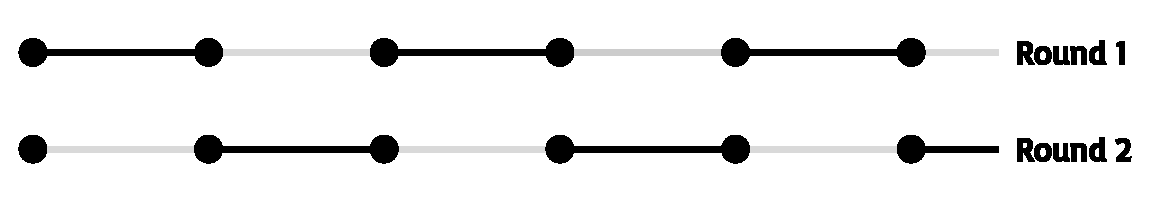
\includegraphics[width=.8\textwidth]{figures/1D/1D_circuit.pdf}
\caption{Qubits in a 1D Lattice. We alternate between two rounds and each round corresponds to a depth of 1. Black dots represent qubits, black lines represent random two qubit gates, grey lines represent inactive gates. }
\label{fig_1d}
\end{figure}
\begin{figure}[!htb]
\centering
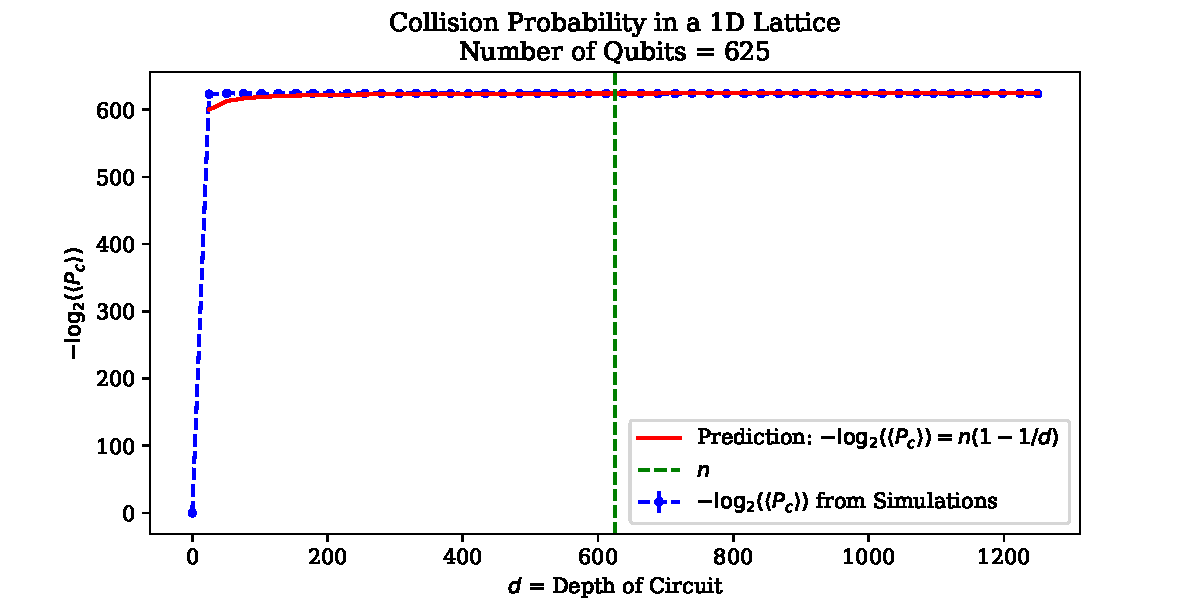
\includegraphics[width=.8\textwidth]{figures/1D/cp_mean_log.pdf}
\caption{$-\log_2(\langle P_c \rangle)$ as a function of $d$ in a 1D lattice with $n = 625$ qubits.}
\label{k_1d} 
\end{figure}
\begin{figure}[!htb]
\centering
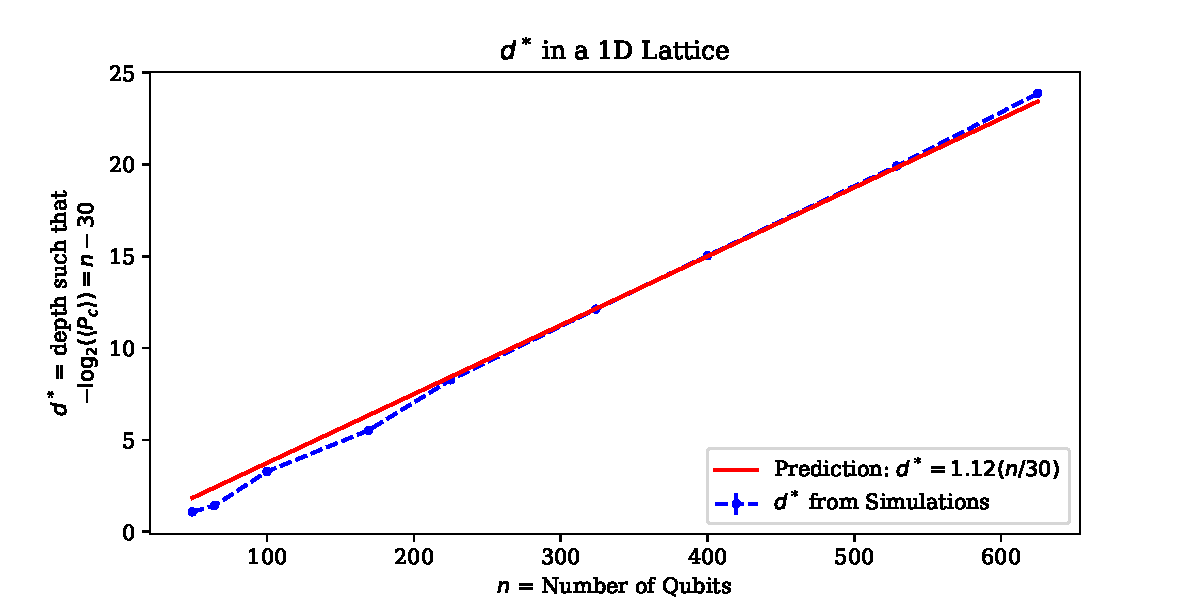
\includegraphics[width=.8\textwidth]{figures/1D/x_star_30.pdf}
\caption{$d^*$ as a function of $n$ in a 1D lattice.}
\label{d_star_1d}
\end{figure}

We would like to note here that in the 1D lattice we did not compute the collision probability at each depth. Rather, we only computed the collision probability for 50 different values of the depth, which were approximately evenly spaced. The reasoning for this is two-fold. First, computing the collision probability given a tableau is the most expensive operation in our simulations. Second, in the 1D lattice, we needed to compute the collision probability for large values of depth on the order of $O(n)$. Likewise, limiting the number of data points we collected saved a significant amount of time while running our simulations.

We see that the numerical results obtained from our simulations support Conjecture {\ref{conjecture_1}}, which predicts 
\begin{equation}
-\log_2(\langle P_c \rangle) = n \left( 1 - O\left(\frac{1}{d} \right) \right) 
\end{equation}
Moreover, for a 1D lattice, we would expect the circuit to saturate at a depth of $d \sim n$. Likewise, looking at Figure {\ref{k_1d}}, it is clear that we will have $-\log_2(\langle P_c \rangle) = O(n - n/d)$ and the circuit clearly saturates well before $d = n$.

To provide further evidence in support of Conjecture {\ref{conjecture_1}}, we define $d^*$ to be the depth such that $-\log_2(\langle P_c \rangle)= n - 30$. Likewise, if we let $O(1/d) = c/d$ for some constant $c$, the conjecture predicts 
\begin{equation}
  -\log_2(\langle P_c \rangle) = n \left( 1 - \frac{c}{d^*} \right) = n - 30
  \quad \Rightarrow \quad
  d^* = c \left( \frac{n}{30} \right) 
\end{equation}
In Figure {\ref{d_star_1d}} we have plotted $d^*$ as a function of $n$ and chosen a value of $c$ that fits the data well. As we can see, the values of $d^*$ computed from our simulations show a clear linear trend, meaning our simulations in a 1D lattice largely agree with the predictions of Conjecture {\ref{conjecture_1}}. 

\subsection{2D Lattice}
The pairs of qubits in a 2D lattice that correspond to a depth of $1$ can be seen in Figure {\ref{fig_2d}}. Similar to the 1D lattice, we perform a round robin cycling through four different rounds when applying our sets of two qubit gates. Each round in this round robin increases the depth of the circuit by $1$. Figure {\ref{k_2d}} shows our results for $-\log_2(\langle P_c \rangle)$ as a function of depth in a 2D lattice with $n=900$. 

\begin{figure}[!htb]
\centering
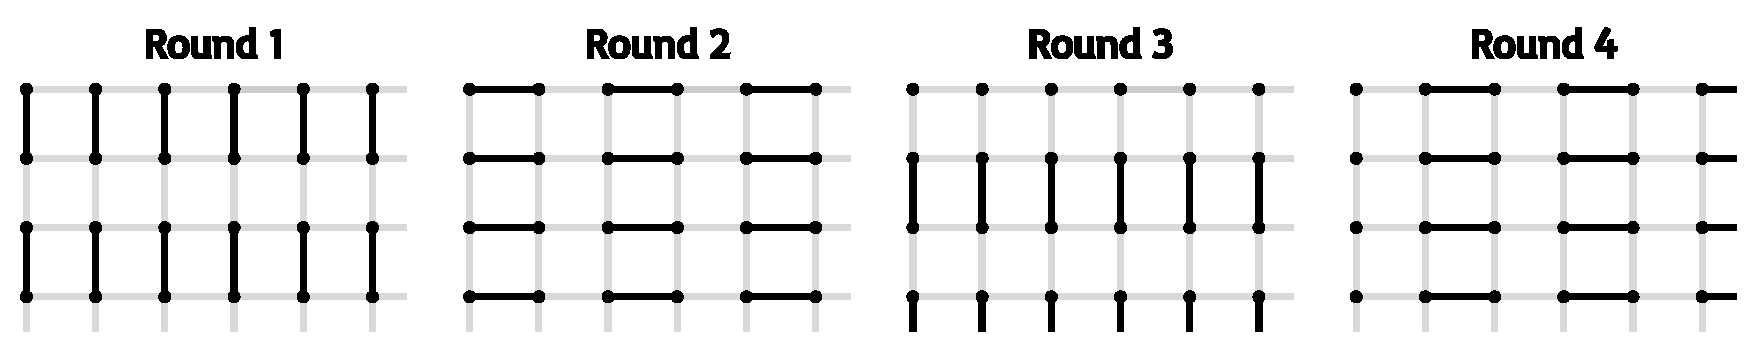
\includegraphics[width=.9\textwidth]{figures/2D/2D_circuit.pdf}
\caption{Qubits in a 2D Lattice. We cycle through four rounds and each round corresponds to a depth of 1. Black dots represent qubits, black lines represent random two qubit gates, grey lines represent inactive gates.}
\label{fig_2d}
\end{figure}
\begin{figure}[!htb]
\centering
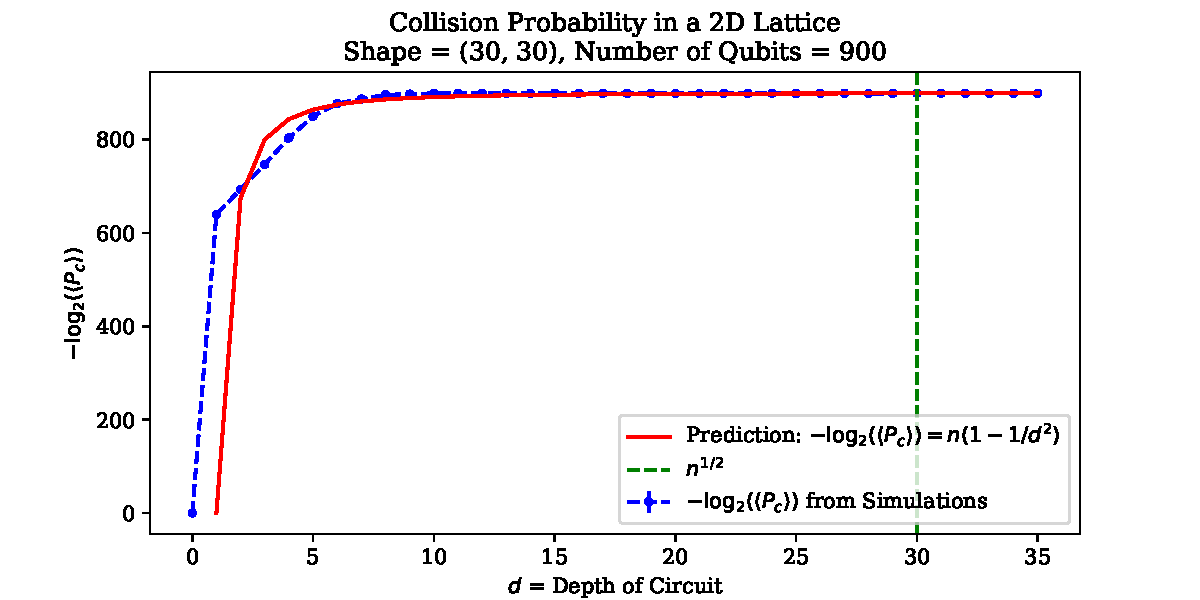
\includegraphics[width=.8\textwidth]{figures/2D/cp_mean_log.pdf}
\caption{$-\log_2(\langle P_c \rangle)$ as a function of $d$ in a 2D lattice with $n = 900$ qubits.}
\label{k_2d}
\end{figure}
\begin{figure}[!htb]
\centering
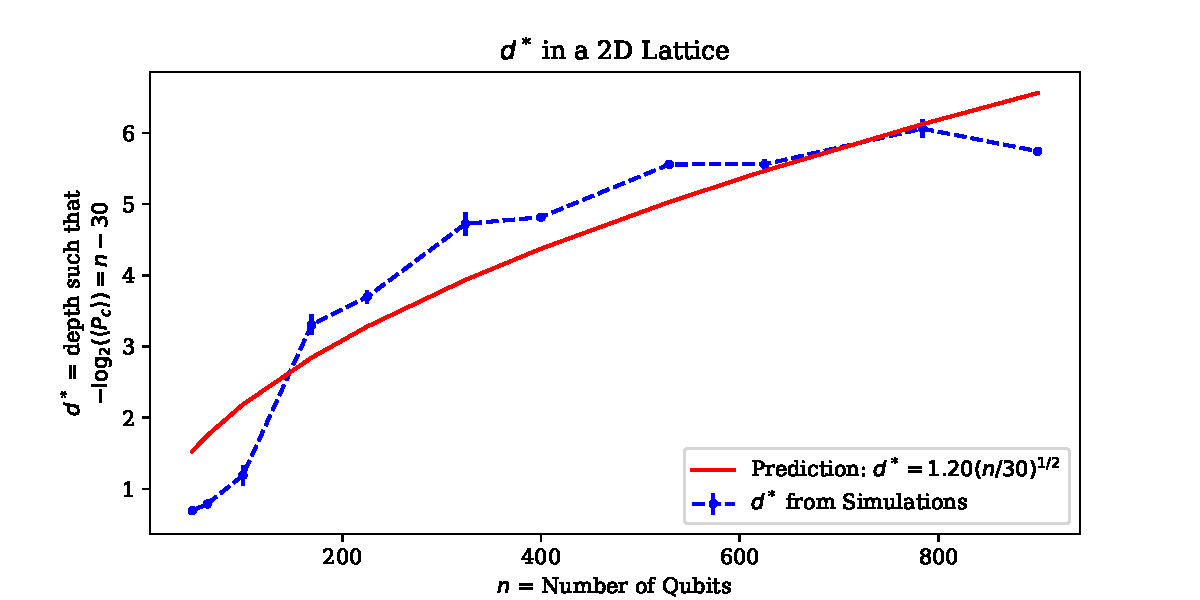
\includegraphics[width=.8\textwidth]{figures/2D/x_star_30.pdf}
\caption{$d^*$ as a function of $n$ in a 2D lattice.}
\label{d_star_2d} 
\end{figure}  

In Figure {\ref{k_2d}}, we collect $36$ data points corresponding to the values of depth $d = 0, 1, 2, \ldots, 35$ so that we can see how $-\log_2(\langle P_c \rangle)$ behaves as a function of $d$ for depths on the order of $O(n^{1/2})$.  

For a 2D lattice, Conjecture {\ref{conjecture_1}} predicts 
\begin{equation}
-\log_2(\langle P_c \rangle) = n \left( 1 - O\left(\frac{1}{d^2} \right) \right) 
\end{equation}
We also expect that for a 2D lattice the circuit will saturate at a depth of $d \sim n^{1/2}$. Looking at Figure {\ref{k_2d}}, we can see that $-\log_2(\langle P_c \rangle) = O(n - n/d^2)$ and the circuit saturates before $d = n^{1/2}$. However, for small values of $d$, we see that the prediction provides a somewhat loose upper bound. Likewise, Conjecture {\ref{conjecture_1}} can likely be modified to provide a tighter bound for small values of $d$. 

Again, to provide further evidence for Conjecture {\ref{conjecture_1}}, we look at how $d^*$ changes as a function of $n$. In this case, the conjecture predicts
\begin{equation}
  -\log_2(\langle P_c \rangle) = n \left( 1 - \frac{c}{{(d^*)}^2} \right) = n - 30
  \quad \Rightarrow \quad
  d^* = c^{1/2} {\left( \frac{n}{30} \right)}^{1/2}
\end{equation}
In Figure {\ref{d_star_2d}}, we have plotted $d^*$ as a function of $n$ in a 2D lattice. Here, we have chosen a value for $c^{1/2}$ that fits the data well. We see that the data collected from our simulations roughly behaves like $n^{1/2}$. However, the data seems to be a bit noisy and it may be the case that a different shaped curve will fit the data better. Modifications to Conjecture {\ref{conjecture_1}} that provide tighter bounds for smaller depth will likely address this issue. Nonetheless, Conjecture {\ref{conjecture_1}} still provides a meaningful upper bound and asymptotic behavior that largely agree with our data. 

\subsection{3D Lattice}
The pairs of qubits in a 3D lattice that correspond to a depth of $1$ can be seen in Figure {\ref{fig_3d}}. Analogous to the 2D lattice, we perform a round robin cycling through six rounds and each round increases the depth of the circuit by $1$. Figure {\ref{k_3d}} shows our result for $-\log_2(\langle P_c \rangle)$ as a function of depth in a 3D lattice with $n = 1000$. 

\begin{figure}[!htb]
\centering
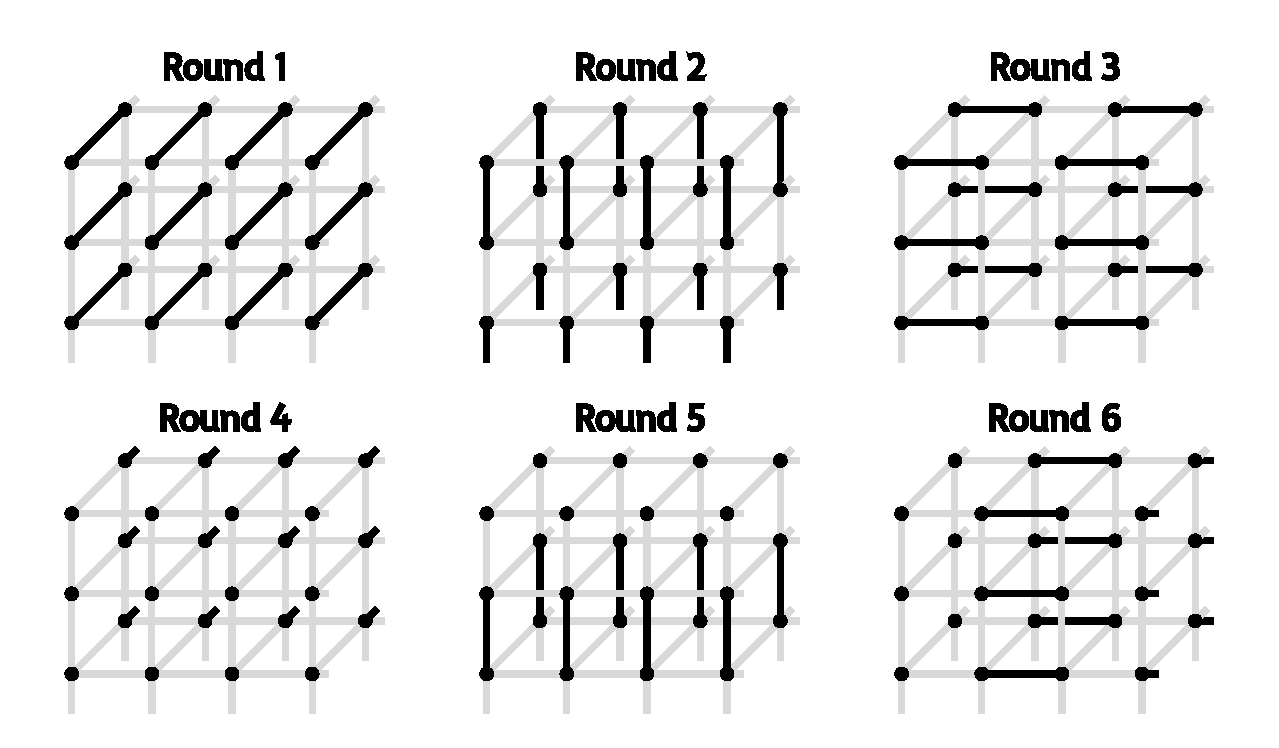
\includegraphics[width=.8\textwidth]{figures/3D/3D_circuit.pdf}
\caption{Qubits in a 3D Lattice. We cycle through six rounds and each round corresponds to a depth of 1. Black dots represent qubits, black lines represent random two qubit gates, grey lines represent inactive gates. }
\label{fig_3d}
\end{figure}
\begin{figure}[!htb]
\centering
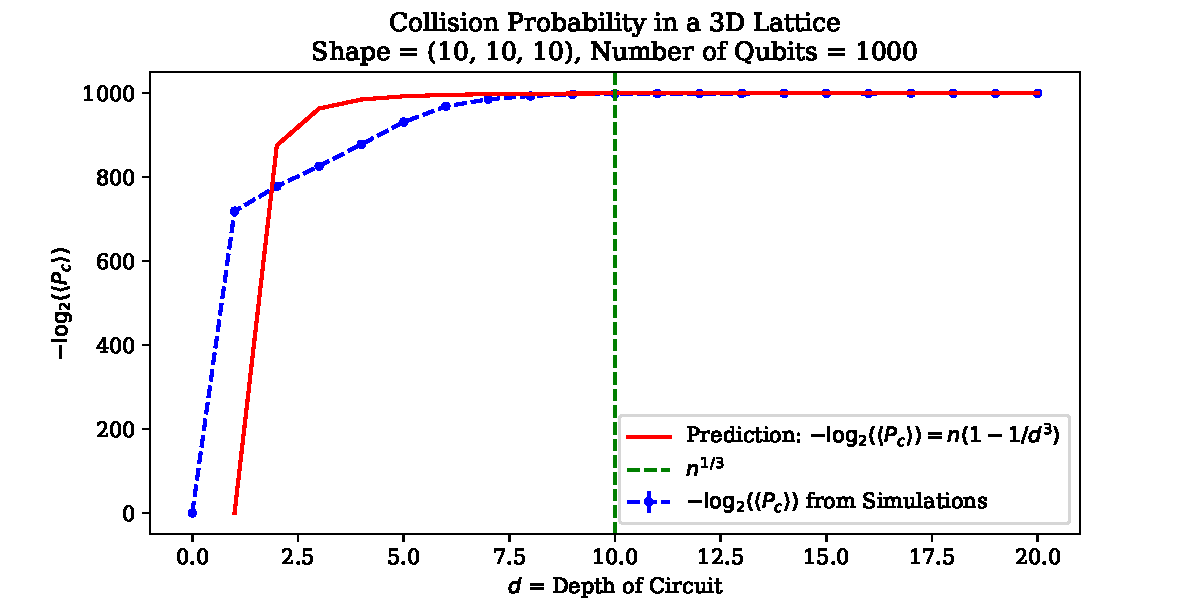
\includegraphics[width=.8\textwidth]{figures/3D/cp_mean_log.pdf}
\caption{$-\log_2(\langle P_c \rangle)$ as a function of $d$ in a 3D lattice with $n = 1000$ qubits.}
\label{k_3d}
\end{figure}
\begin{figure}[!htb]
\centering
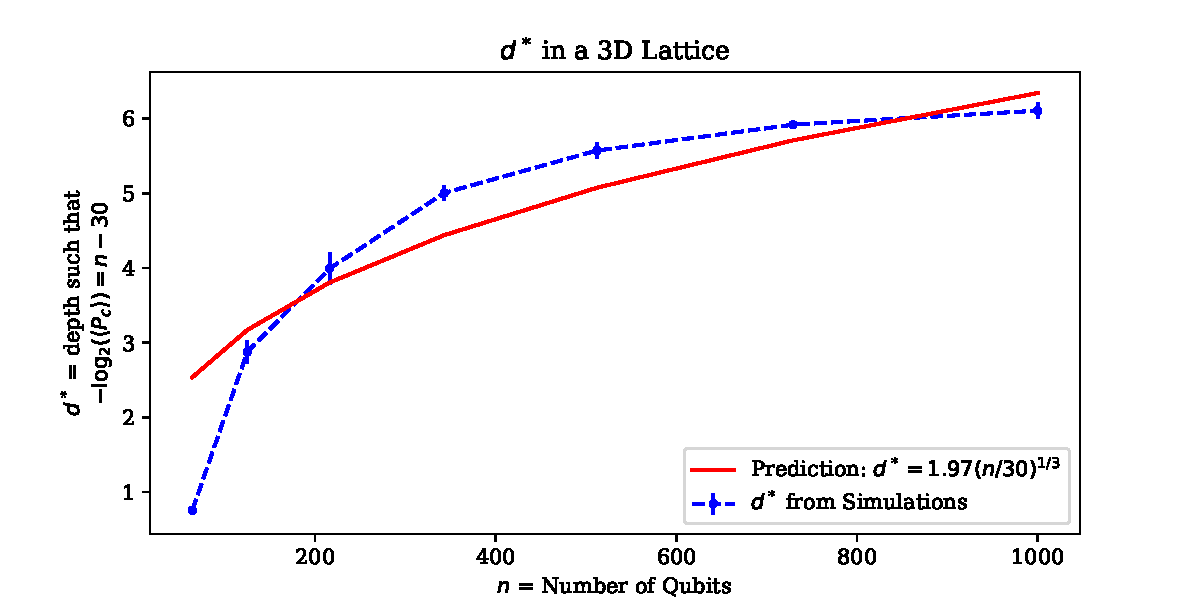
\includegraphics[width=.8\textwidth]{figures/3D/x_star_30.pdf}
\caption{$d^*$ as a function of $n$ in a 3D lattice with $m = 25$.}
\label{d_star_3d} 
\end{figure} 

In Figure {\ref{k_3d}}, we collect $21$ data points corresponding to the values of depth $d = 0, 1, 2, \ldots, 20$ so that we can see how $-\log_2(\langle P_c \rangle)$ behaves as a function of $d$ for depths on the order of $O(n^{1/3})$.

For a 3D lattice, Conjecture {\ref{conjecture_1}} predicts
\begin{equation}
-\log_2(\langle P_c \rangle) = n \left( 1 - O\left(\frac{1}{d^3} \right) \right) 
\end{equation}
We also expect that for a 3D lattice the circuit will saturate at a depth of $d \sim n^{1/3}$. Looking at Figure {\ref{k_3d}}, we can see that $-\log_2 (\langle P_c \rangle) = O(n - n/d^3)$ and the circuit tends to saturate around $d = n^{1/3}$. Similar to the case of the 2D lattice, we see that the prediction provides a loose upper bound for small values of $d$. 

We also see how $d^*$ changes as a function of $n$. Here, Conjecture {\ref{conjecture_1}} predicts
\begin{equation}
  -\log_2(\langle P_c \rangle) = n \left( 1 - \frac{c}{{(d^*)}^3} \right) = n - 30
  \quad \Rightarrow \quad
  d^* = c^{1/3} {\left( \frac{n}{30} \right)}^{1/3}
\end{equation}
In Figure {\ref{d_star_3d}}, we have plotted $d^*$ as a function of $n$ and have chosen a value of $c^{1/3}$ that fits the data well. Similar to the case of the 2D lattice, we see that the values of $d^*$ collected from our simulations roughly display a $n^{1/3}$ behavior. However, there may be a better curve that fits the function. Again, we hypothesize that modifications to Conjecture {\ref{conjecture_1}} that provide tighter bounds for small values of $d$ will likely address these issues. 

\subsection{Complete Graph}
In a complete graph, we look at $-\log_2(\langle P_c \rangle)$ as a function of the total number of gates applied to the circuit $N$. Likewise, we simply choose two qubits uniformly at random and apply a gate to those two qubits. After doing so, $N$ increases by $1$. An illustration of this process can be seen in Figure {\ref{fig_cg}}. Figure {\ref{k_cg}} shows our results for $-\log_2(\langle P_c \rangle)$  as a function of $N$ in a complete graph with $n = 625$. 

\begin{figure}[!htb]
\centering
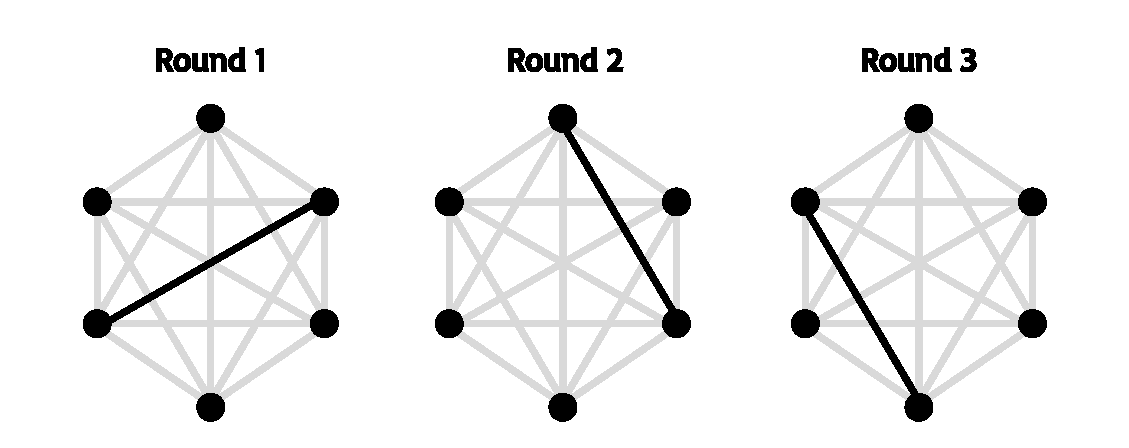
\includegraphics[width=.8\textwidth]{figures/CG/CG_circuit.pdf}
\caption{Qubits in a Complete Graph. This is an illustration of 6 qubits laid out in a complete graph. Each round corresponds to a single gate. In each round, two qubits are chosen uniformly at random. Black dots represent qubits, black lines represent random two qubit gates, grey lines represent inactive gates. }
\label{fig_cg}
\end{figure}
\begin{figure}[!htb]
\centering
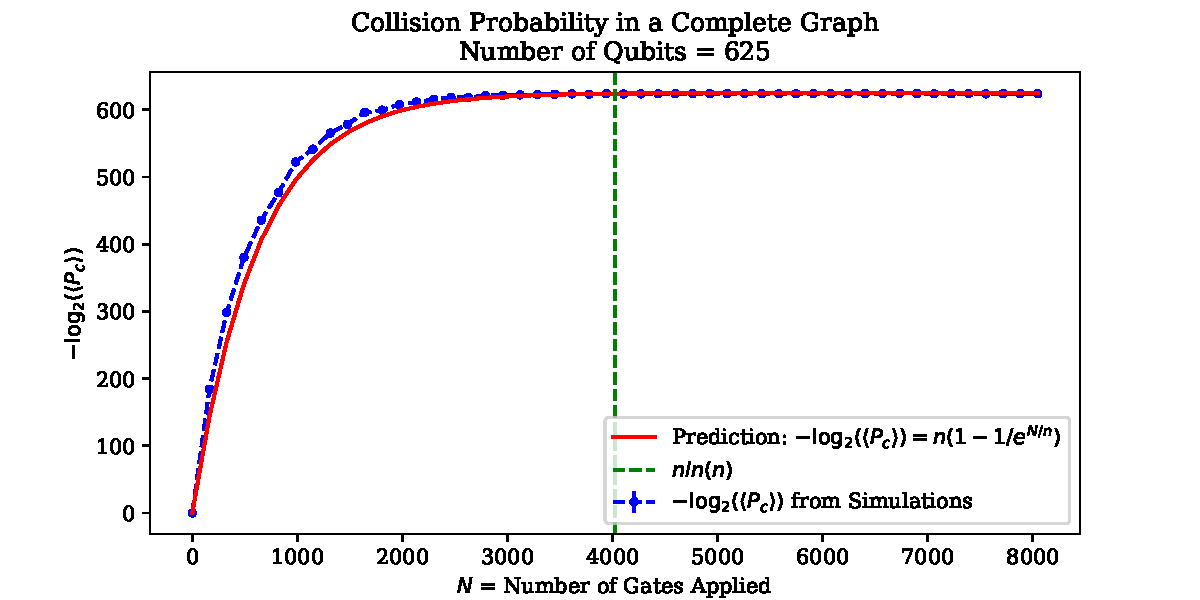
\includegraphics[width=.8\textwidth]{figures/CG/cp_mean_log.pdf}
\caption{$-\log_2(\langle P_c \rangle)$ as a function of $N$ in a complete graph with $n = 625$ qubits.}
\label{k_cg}
\end{figure}
\begin{figure}[!htb]
\centering
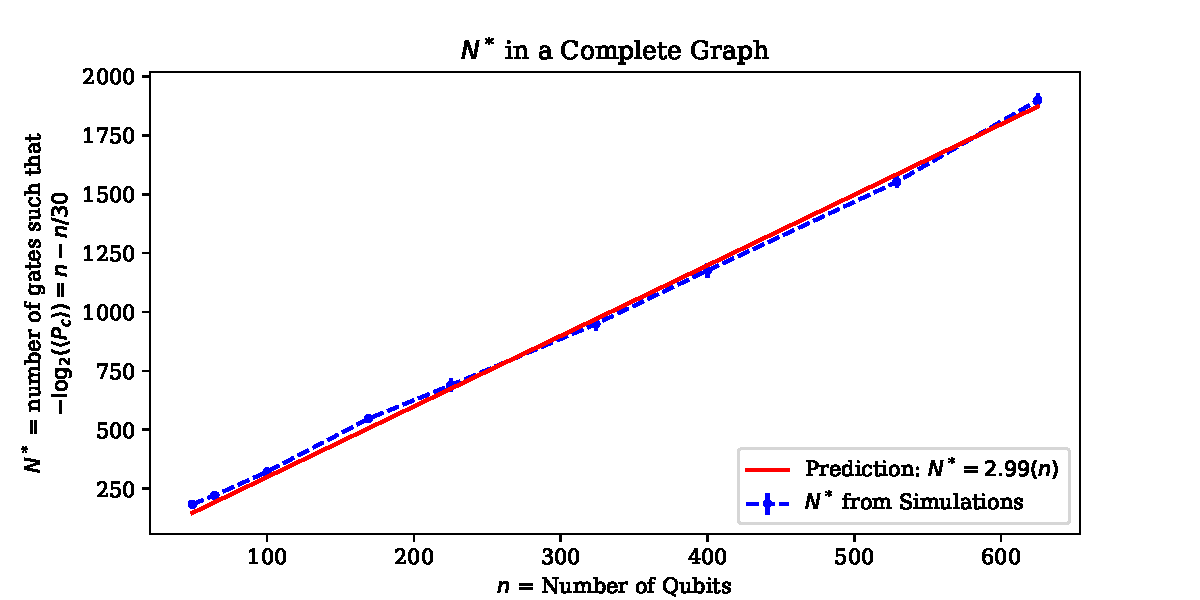
\includegraphics[width=.8\textwidth]{figures/CG/x_star_30.pdf}
\caption{$N^*$ as a function of $n$ in a complete graph.}
\label{N_star_cg} 
\end{figure}

Similar to the 1D lattice, we have also chosen to only compute the collision probability for $50$ different values of $N$. The reasons for doing this are the same as those described in Section {\ref{1d_lattice}}. These $50$ data points are also approximately evenly space out and we look at the number of gates $N$ on the order of $n \ln(n)$.

We see that the numerical results obtained from our simulations support Conjecture {\ref{conjecture_2}}, which predicts
\begin{equation}
-\log_2(\langle P_c \rangle) = n \left( 1 - O\left(\frac{1}{e^{N/n}} \right) \right) 
\end{equation}
This conjecture also predicts that the circuit will saturate around $N \sim n \ln(n)$. Looking at Figure {\ref{k_cg}}, we see that $-\log_2(\langle P_c \rangle)= O(n - n / e^{N/n})$ and the circuit saturates around $N = n \ln(n)$.

Similar to the 1D, 2D, and 3D lattices, we provide further support for Conjecture {\ref{conjecture_2}} by defining a new quantity $N^*$. However, in this case, we define $N^*$ to be the number of gates such that $-\log_2(\langle P_c \rangle)= n - n/30$. Likewise, the conjecture predicts
\begin{equation}
  -\log_2(\langle P_c \rangle)= n \left( 1 - \frac{c}{e^{N^*/n}} \right)
  = n - \frac{n}{30}
  \quad \Rightarrow \quad
  e^{N^*/n} = 30c
  \quad \Rightarrow \quad
  N^* = \ln(30c) (n)  
\end{equation}
In Figure {\ref{N_star_cg}}, we have plotted $N^*$ as a function of $n$. Here, we have adjusted the value of $\ln(30c)$ so the prediction fits the data well. Similar to the case of the 1D lattice, we see a clear linear trend in the values of $N^*$ from our simulations that line up very closely with our prediction. Both Figures {\ref{k_cg}} and {\ref{N_star_cg}} provide data that strongly agrees with the predictions of Conjecture {\ref{conjecture_2}}. Likewise, the upper bounds provided in Conjecture {\ref{conjecture_2}} are quite tight. 


\subsection{Fluctuations in Collision Probability}
So far, we have shown that our numerical results largely support Conjecture {\ref{conjecture_1}} in a 1D lattice and Conjecture {\ref{conjecture_2}} in a complete graph. We have also shown that Conjecture {\ref{conjecture_1} provides meaningful, but loose, upper bounds in a 2D and 3D lattice. Overall, these numerical results are mostly concerned with the expected value of the collision probability $\langle P_c \rangle$. In this section, we present some numerical results concerned with the standard deviation of the collision probability $\Delta P_c$.

Figures {\ref{fig_1d_std}}, {\ref{fig_2d_std}}, {\ref{fig_3d_std}}, and {\ref{fig_cg_std}} show our numerical results for $-\log_2 (\Delta P_c)$ in a 1D lattice, 2D lattice, 3D lattice, and complete graph respectively. These plots show how $-\log_2 (\Delta P_c)$ changes as a function of depth for fixed values of $n$. 

\begin{figure}[!htb]
\centering
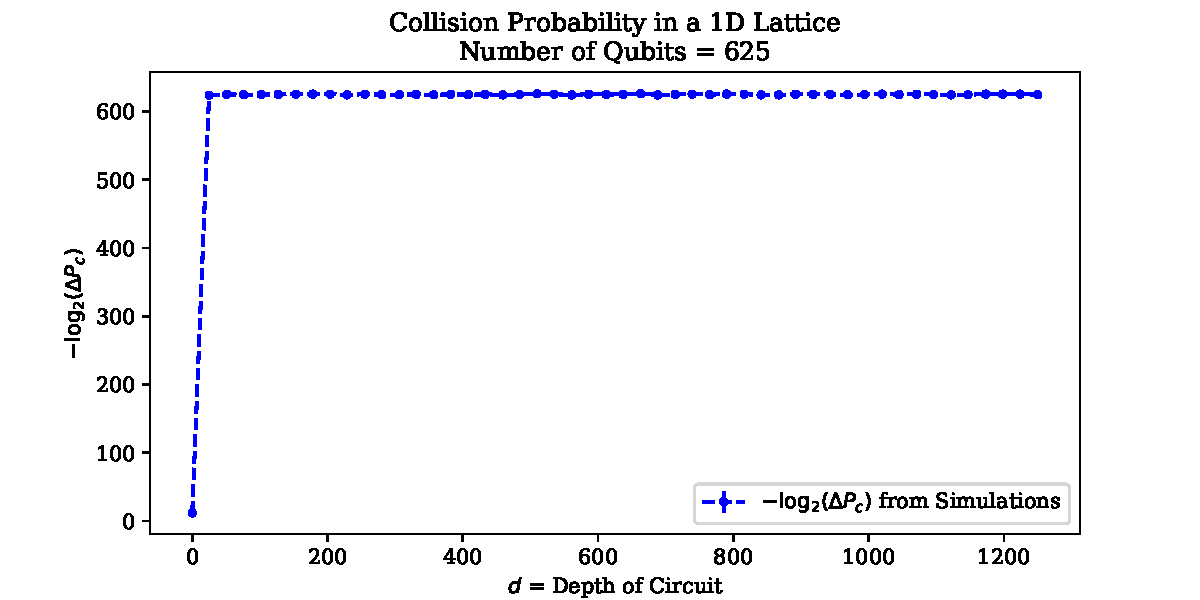
\includegraphics[width=.8\textwidth]{figures/1D/cp_std_log.pdf}
\caption{$-\log_2(\Delta P_c)$ as a function of $d$ in a 1D lattice with n = 625 qubits.}
\label{fig_1d_std}
\end{figure}
\begin{figure}[!htb]
\centering
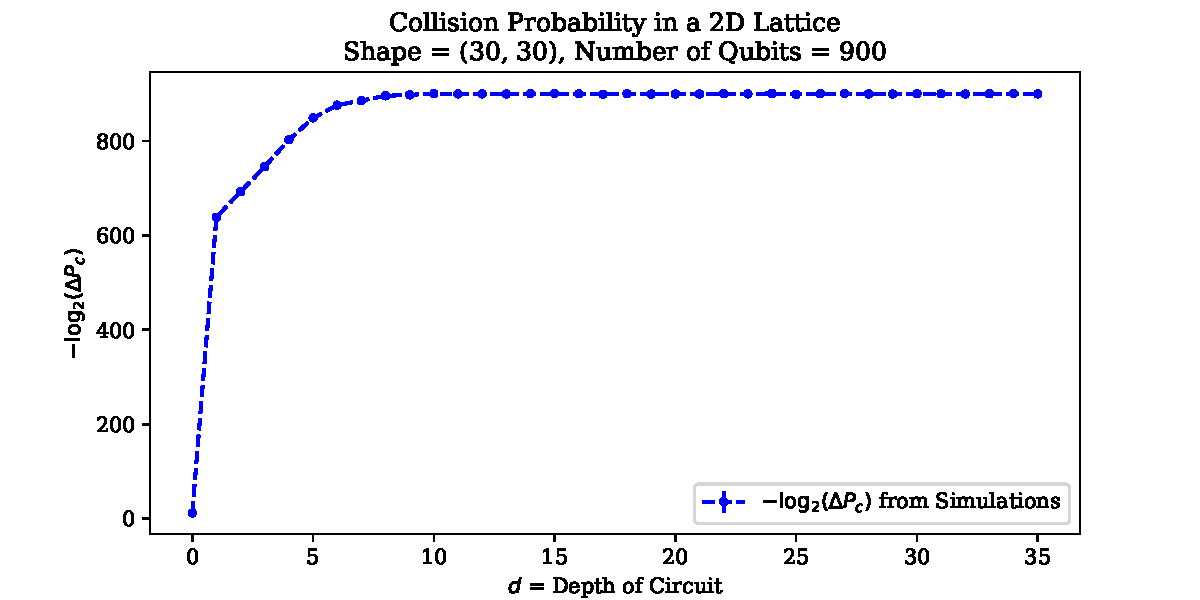
\includegraphics[width=.8\textwidth]{figures/2D/cp_std_log.pdf}
\caption{$-\log_2(\Delta P_c)$ as a function of $d$ in a 2D lattice with n = 900 qubits.}
\label{fig_2d_std}
\end{figure}
\begin{figure}[!htb]
\centering
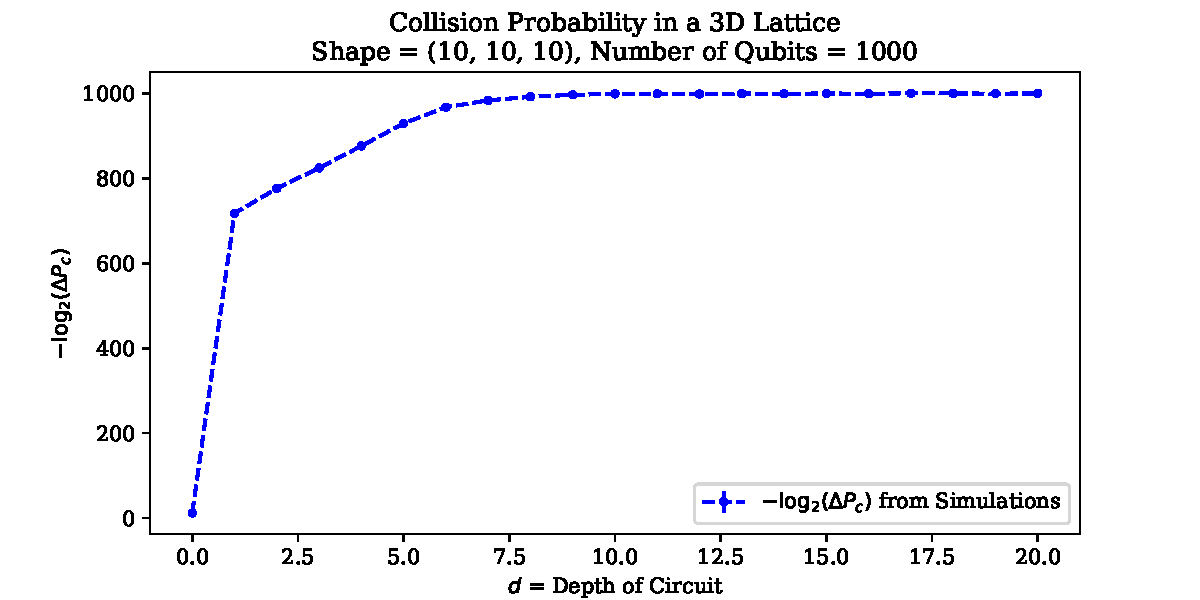
\includegraphics[width=.8\textwidth]{figures/3D/cp_std_log.pdf}
\caption{$-\log_2(\Delta P_c)$ as a function of $d$ in a 3D lattice with n = 1000 qubits.}
\label{fig_3d_std}
\end{figure}
\begin{figure}[!htb]
\centering
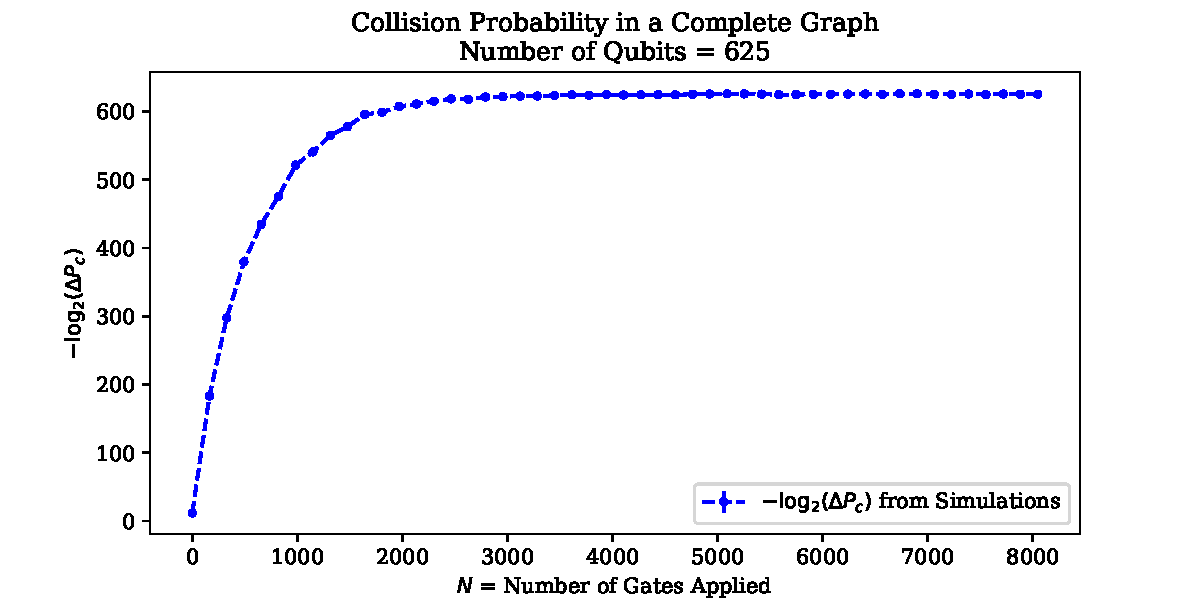
\includegraphics[width=.8\textwidth]{figures/CG/cp_std_log.pdf}
\caption{$-\log_2(\Delta P_c)$ as a function of $d$ in a complete graph with n = 625 qubits.}
\label{fig_cg_std}
\end{figure}
\begin{figure}[!htb]
\centering
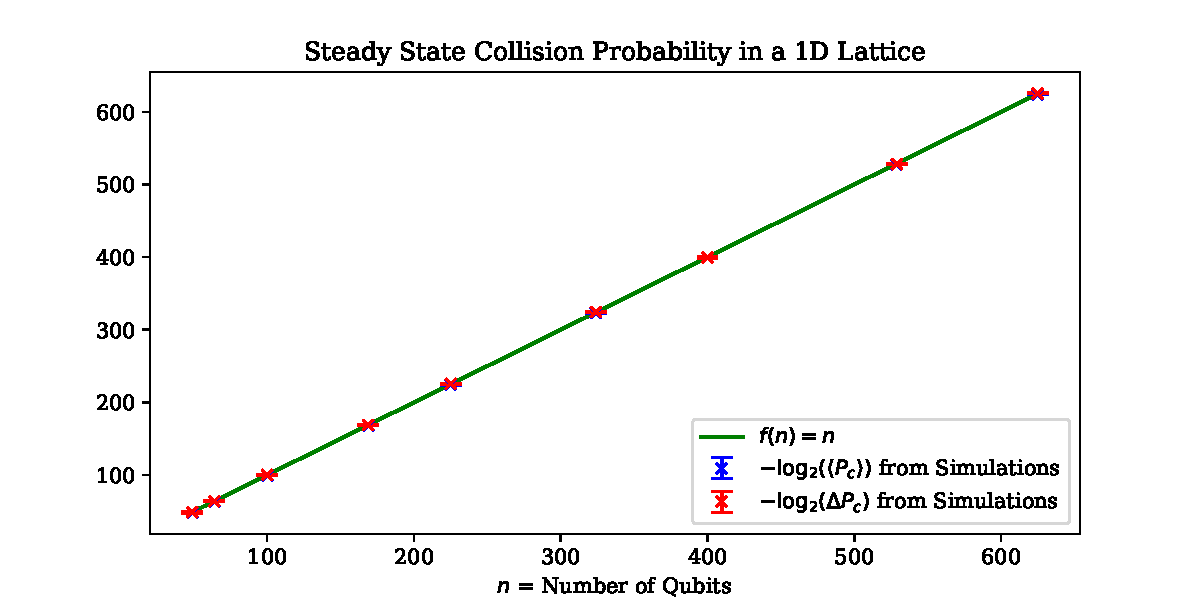
\includegraphics[width=.8\textwidth]{figures/1D/steady_state_cp.pdf}
\caption{$-\log_2(\langle P_c \rangle)$ and $-\log_2(\Delta P_c)$ as a function of $n$ in a 1D lattice at saturated depths.}
\label{fig_steady_state}
\end{figure}

We see some striking similarities when comparing Figures {\ref{fig_1d_std}}, {\ref{fig_2d_std}}, {\ref{fig_3d_std}}, and {\ref{fig_cg_std}} with Figures {\ref{k_1d}}, {\ref{k_2d}}, {\ref{k_3d}}, {\ref{k_cg}} respectively. That is, the data collected from our simulations suggest that the values of $-\log_2(\langle P_c \rangle)$ and $-\log_2(\Delta P_c)$ grow similarly as functions of depth and number of qubits.
    
Furthermore, in Figure {\ref{fig_steady_state}} we plot both $-\log_2(\langle P_c \rangle)$ and $-\log_2(\Delta P_c)$ as a function of $n$ in a 1D lattice. In these plots, we have chosen large depths for each value of $n$ so that the circuits have been fully saturated. We see that both $-\log_2(\langle P_c \rangle)$ and $-\log_2(\Delta P_c)$ are almost exactly equal to $n$ when the circuits have reached a steady state. Moreover, although not included in this paper, we have found nearly the same exact results when creating the same plots for a 2D and 3D lattice as well as in a complete graph. 

These results are quite interesting as they imply that as a circuit saturates, we expect fluctuations in the collision probability to be approximately $\Delta P_c \approx {(1/2)}^n$. This means that the steady state fluctuations in the collision probability become exponentially small as the size of the circuit grows. 

\subsection{Summary of the Numerical Results}
We have tested Conjectures {\ref{conjecture_1}} and {\ref{conjecture_2}} on three separate accounts: the behavior of $-\log_2 (\langle P_c \rangle)$ as function of $d$ or $N$, the depths or number of gates at which the circuits saturate, and the behavior of $d^*$ or $N^*$ as a function of $n$. Overall, we found that our data strongly agrees with the predictions of Conjecture {\ref{conjecture_1}} in a 1D lattice and Conjecture {\ref{conjecture_2}} in a complete graph.

We found that our data roughly agreed with Conjecture {\ref{conjecture_1}} in a 2D and 3D lattice. Specifically, we saw that the upper bounds provided by the conjecture seemed a bit loose for small values of depth. Likewise, we hypothesize that modifications to Conjecture {\ref{conjecture_1}} will likely be able to address these issues. Nonetheless, our data still suggests that Conjecture {\ref{conjecture_1}} provides meaningful upper bounds for a 2D and 3D lattice. 

Lastly, we diverged slightly from our original conjectures to discuss fluctuations we observed in the collision probability. Our numerical results suggest that $-\log_2(\langle P_c \rangle)$ and $-\log_2(\Delta P_c)$ grow similarly as functions of depth and number of qubits. We also observed that the standard deviation of the collision probability $\Delta P_c \approx {(1/2)}^n$ for large depths where the circuit is saturated, regardless of its geometry.

\section{Conclusion} 
Throughout this paper, our main focus has been on studying one statistical property of pseudo-random quantum circuits: how the expected value of the collision probability behaves as a function of the depth of the circuit and the number of qubits in the circuit. In doing so, we began by introducing Conjectures {\ref{conjecture_1}} and {\ref{conjecture_2}}, which we have tested numerically via simulations of pseudo-random quantum circuits. Before presenting the structure and results of our simulations, we described some of the mathematical principles allowing us to efficiently simulate quantum circuits composed only of Clifford Gates. We also presented an algorithm to efficiently compute the collision probability of such circuits.

Overall, our numerical results for a 1D lattice and a complete graph strongly agree with the predictions made by Conjectures {\ref{conjecture_1}} and {\ref{conjecture_2}} respectively. Our numerical results also suggest that Conjecture {\ref{conjecture_1}} likely provides meaningful, but somewhat loose, upper bounds for a 2D and 3D lattice. We also found that $-\log_2(\langle P_c \rangle)$ and $-\log_2(\Delta P_c)$ behave similarly as functions of depth and number of qubits and that steady state fluctuations in the collision probability are approximately $\Delta P_c \approx {(1/2)}^n$.

\bibliography{mybib}

\end{document}
%%% Local Variables:
%%% mode: latex
%%% TeX-master: t
%%% End:


